
%%%%%%%%%%%%%%%%%%%%%%%%%%%%%%%%%%%%%%%%%%%%%%%%%%%%%%%%%%%%%%%%%%%%%%%%
%Para las ecuaciones siempre es Ec.(n).
%Para las figuras siempre es Fig.n, incluso en el caption de la figura. Tambien las Tablas
%Para las referencias es [n]
%%%%%%%%%%%%%%%%%%%%%%%%%%%%%%%%%%%%%%%%%%%%%%%%%%%%%%%%%%%%%%%%%%%%%%%%

\documentclass[
reprint,
%notitlepage,
%superscriptaddress,
%groupedaddress,
%unsortedaddress,
%runinaddress,
%frontmatterverbose, 
%preprint,
%showpacs,preprintnumbers,
%nofootinbib,
%nobibnotes,
%bibnotes,
%11 pt,
amsmath,
amssymb,
aps,
pra,
%prb,
%rmp,
%tightenlines %esto hizo el milagro de sacar los espacios en blancos estocásticos (?)
 %prstab,
%prstper,
%floatfix,\textbf{}
]{revtex4-1} %Instalar primero para usarlo. Paquete malo.

%\documentclass[onecolumn, aps, amsmath,amssymb ]{article}
\usepackage{lipsum}  
\usepackage{graphicx}% Include figure files
\usepackage{subfig}
\usepackage{braket}
\usepackage{comment} %comment large chunks of text
\usepackage{dcolumn}% Align table columns on decimal point
\usepackage{bm}% bold math
%\usepackage{hyperref}% add hypertext capabilities
\usepackage[mathlines]{lineno}% Enable numbering of text and display math
%\linenumbers\relax % Commence numbering lines
\usepackage{mathtools} %% Para el supraíndice

\usepackage[nice]{nicefrac}

%%%%%%%El Señor Español%%%%%%%%%%%%%%%%%%%%%%%%%%%
\usepackage[utf8]{inputenc} %acento
\usepackage[
spanish, %El lenguaje.
es-tabla, %La tabla y no cuadro.
activeacute, %El acento.
es-nodecimaldot %Punto y no coma con separador de números
]{babel}
\usepackage{microtype} %para hacerlo más bonito :33 como vos (?) 
%%%%%%%%%%%%%%%%%%%%%%%%%%%%%%%%%%%%%%%%%%%%%%%%%%%
%%%%%%%%% Para que las imágenes se queden dónde las quiero (?
\usepackage{float}
%%%%%%%%%%

%%%%%%%%Cambia a Fig de Figure%%%%%%%%%%
\makeatletter
\renewcommand{\fnum@figure}{Fig. \thefigure} 
\makeatother
%%%%%%%%%%%%%%%%%%%%%%%%%%%%%%%%%%%%%%%%
\raggedbottom


\begin{document}
%%%%%%%%%%%%%%%%%%%%%%%%%%%%%%%%%%Título%%%%%%%%%%%%%%%%%%%%%%%%%%%%%%%%%%%%%%
%%%%%%%%%%%%%%%%%%%%%%%%%%%%%%%%%%%%%%%%%%%%%%%%%%%%%%%%%%%%%%%%%%%%%%%%%%%%%%

\title{Práctica 4: Aprendizaje supervisado en redes multicapa}
\author{Evelyn~G.~Coronel}

\affiliation{
Redes Neuronales - Instituto Balseiro}

\date[]{\lowercase{\today}} %%lw para lw, [] sin date

\begin{abstract}
En esta práctica se realiza el aprendizaje supervisado para distintas arquitecturas y problemas usando el algoritmo de retropropagación.
\end{abstract} 
\maketitle
%%%%%%%%%%%%%%%%%%%%%%%%%%%%%%%%%%%%%%%%%%%%%%%%%%%%%%%%%%%%%%%%%%%%%%%%%%%%%%%%%%%
% Podemos usar cualquiera de los dos comandos: \input o \include para incluir el texto
%\input{./Capitulo1/cap1.tex}

\section*{Ejercicio 1: XOR}

\subsection*{Casos base para el entrenamiento}

Para este problema básico, usamos todos los casos posibles para el entrenamiento, es decir, no tenemos ejemplos para verificar la red neuronal. Estos casos se presentan en la Tabla\,\ref{tab:xor}.

\begin{table}[H]
\centering
\begin{tabular}{r | r | r}
Entrada 1 & Entrada 2 & Salida 	\\ \hline
-1 		  &-1	& +1 \\
-1 		  &+1	& -1\\
-1 		  &-1	& -1\\
+1 		  &+1	& +1\\
\end{tabular}
\caption{Todos los casos posibles para la función XOR.} \label{tab:xor}
\end{table}

Se utilizaron dos arquitecturas para el algoritmos de retropropagación, además de agregar una neuronas adicionales para simular los umbrales. La función de transferencia para la salida fue $\tanh({x})$ y la función error que se minimiza es la función error cuadrático medio. En todas las simulaciones se usó un \emph{learning rate} $\eta=0.05$, que cuantifica el cambio de los pesos en función de las épocas.

\begin{figure}[H]
    \begin{minipage}{0.24\textwidth}
        \centering
        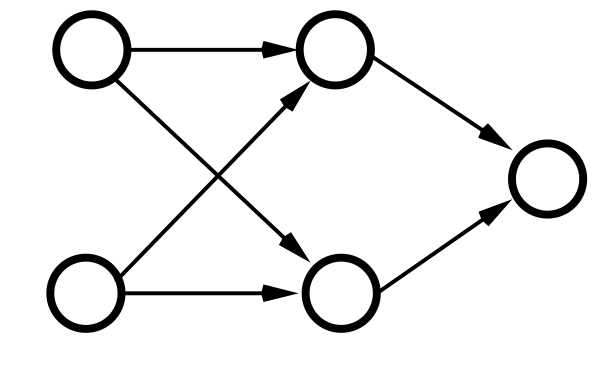
\includegraphics[width=0.8\textwidth]{ejer_1_221.png} % first figure itself
       \caption{Arquitectura 2-2-1}\label{fig:arq-221}
    \end{minipage}\hfill%
    \begin{minipage}{0.24\textwidth}
        \centering
		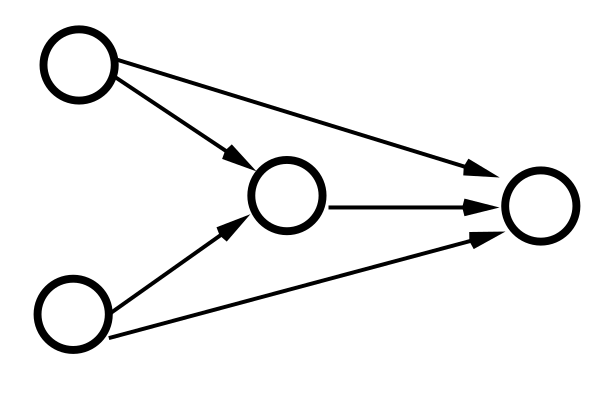
\includegraphics[width=0.75\textwidth]{ejer_1_211.png} % second figure itself
        \caption{Arquitectura 2-1-1} \label{fig:arq-211}
    \end{minipage}
\end{figure}


%\begin{figure}[H]
%	{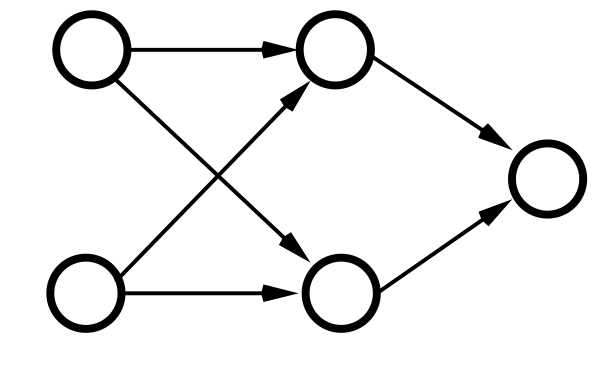
\includegraphics[width=0.2\textwidth]{ejer_1_221.png} }{\caption{Arquitectura 2-2-1}\label{fig:arq-221}}
%	{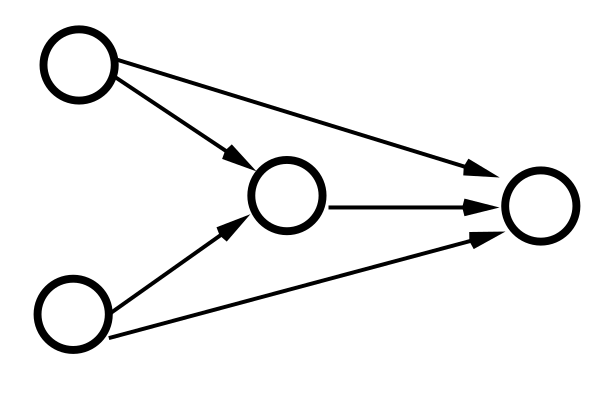
\includegraphics[width=0.2\textwidth]{ejer_1_211.png}}{\caption{Arquitectura 2-1-1} 	\label{fig:arq-211}}
	%\caption{Las arquitecturas utilizadas para el regresionar la función XOR} \label{fig:ej_1}
%\end{figure}

\subsection*{Arquitectura 2-2-1}

Un esquema de la arquitectura utilizada en este caso se muestra en la Fig.\,\ref{fig:arq-221}. En la misma se observa dos entradas, una capa oculta con 2 neuronas conectadas a cada entrada, y una salida conectada a la capa oculta.
%\begin{figure}[H]
%	\centering
%	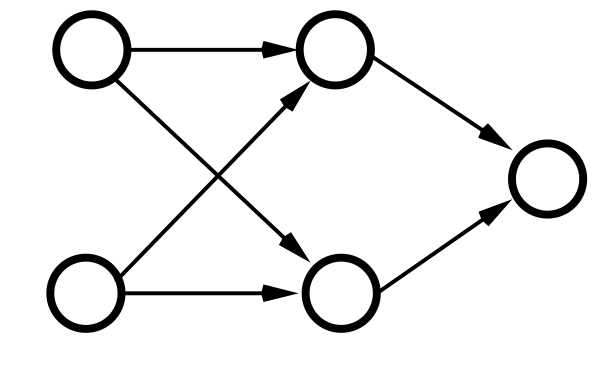
\includegraphics[width=0.25\textwidth]{ejer_1_221.png}
%	\caption{Arquitectura 2-2-1}
%	\label{fig:arq-221}
%\end{figure}

\subsubsection*{Pérdida en función de la época}

La evolución de la pérdida, que en este caso es la función  error cuadrático medio,  para distintas condiciones iniciales para los pesos y el umbrales se muestra en la Fig.\ref{fig:XOR_err_221}. Se observa que en el trial 5 para esta ejecución del programa, convergen a un mínimo local de la función error.

\begin{figure}[H]
	\centering
	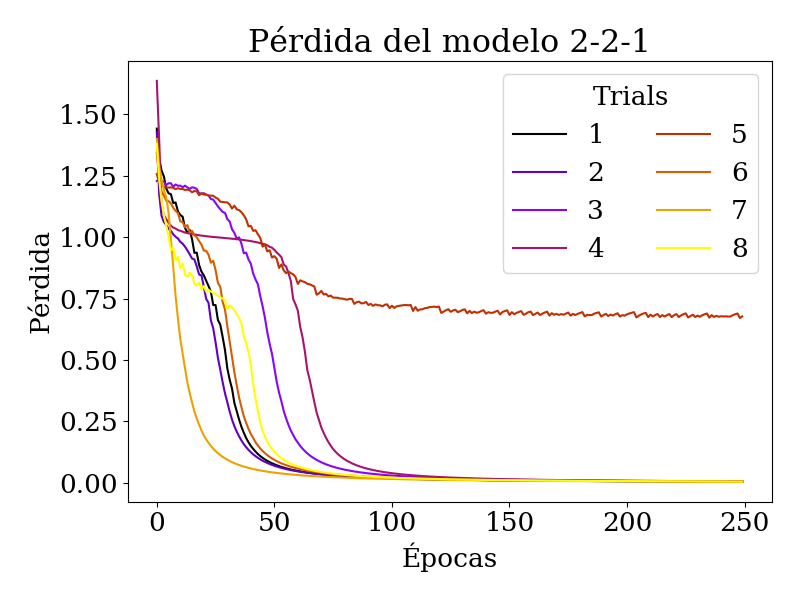
\includegraphics[width=0.45\textwidth]{../Graficos/ejer_1_2-2-1_los.png}
	\caption{Pérdida en función de las épocas para la arquitectura 2-2-1 para el problema del la función XOR para distintas condiciones iniciales.}
	\label{fig:XOR_err_221}
\end{figure}
Si consideramos la exactitud de la red neuronal, se observa que para el trial 5, su valor es de $0.5$. Esto indica que la red neuronal predice la salida del $50\%$ de los casos de entrenamiento, es este caso $2$ ejemplos de $4$  en total.

\begin{figure}[H]
	\centering
	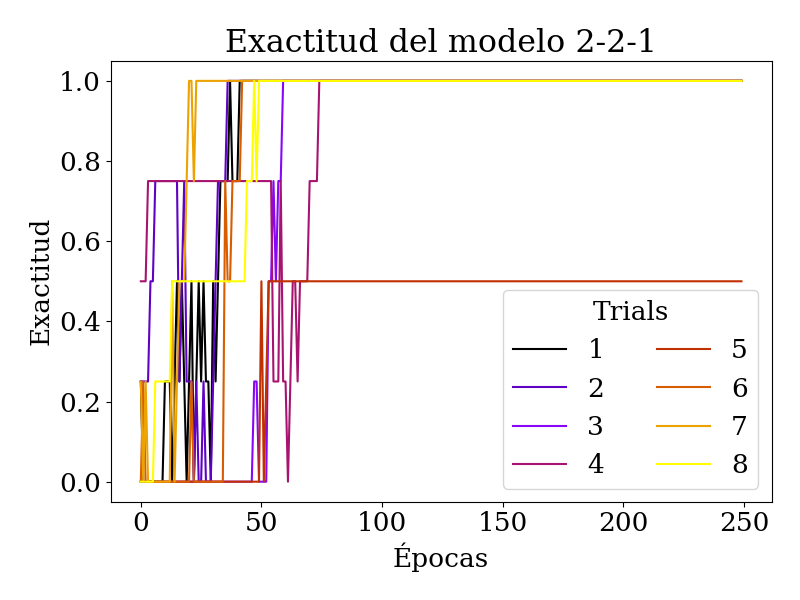
\includegraphics[width=0.45\textwidth]{../Graficos/ejer_1_2-2-1_acc.png}
	\caption{Exactitud en función de las épocas para la arquitectura 2-2-1.}
	\label{fig:XOR_acc_221}
\end{figure}

\subsection*{Arquitectura 2-1-1}
Un esquema de la arquitectura utilizada en esta sección se observa en la Fig.\,\ref{fig:arq-211}. En la misma se observa dos entradas de la función XOR, una capa oculta con 1 neurona conectada a cada entrada, y una salida conectada a la capa oculta además de estar conectada a las entrada de la red.

%\begin{figure}[H]
%	\centering
%	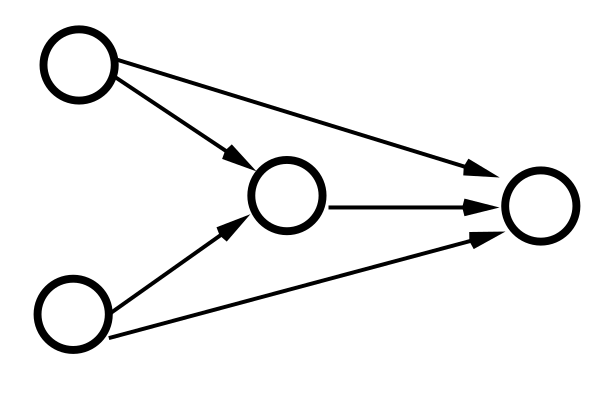
\includegraphics[width=0.2\textwidth]{ejer_1_211.png}
%	\caption{Arquitectura 2-1-1}
%	\label{fig:arq-211}
%\end{figure}
\subsubsection*{Pérdida en función de la época}


La Fig.\,\ref{fig:XOR_err_211} muestra la evolución de la pérdida con las épocas de la ejecución del programa para distintas condiciones iniciales. En la misma se ve como la red converge a una pérdida nula sólo para 3 de los 8 casos en las primeras 250 épocas. Esto se debe a que la cantidad de parámetros que tiene la red para ajustar la función XOR no es suficiente para regresionar la función. La cantidad de parámetros viene dada por la arquitectura del problema.

En la evolución  de la exactitud  con las épocas de la Fig.\,\ref{fig:XOR_acc_211}, muestra que los casos donde no se converge a una solución, la red es capaz  de predecir 3 de los 4 ejemplos usando en el entrenamiento, ya que la exactitud vale $75\%$.

\begin{figure}[H]
	\centering
	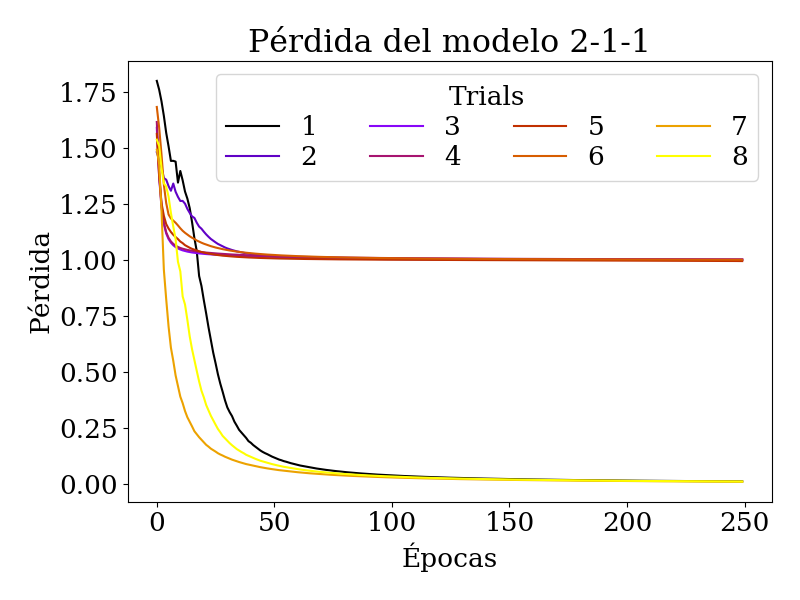
\includegraphics[width=0.44\textwidth]{../Graficos/ejer_1_2-1-1_los.png}
	\caption{Pérdida en función de las épocas para la arquitectura 2-1-1 para el problema del la función XOR.}
	\label{fig:XOR_err_211}
\end{figure}


\begin{figure}[H]
	\centering
	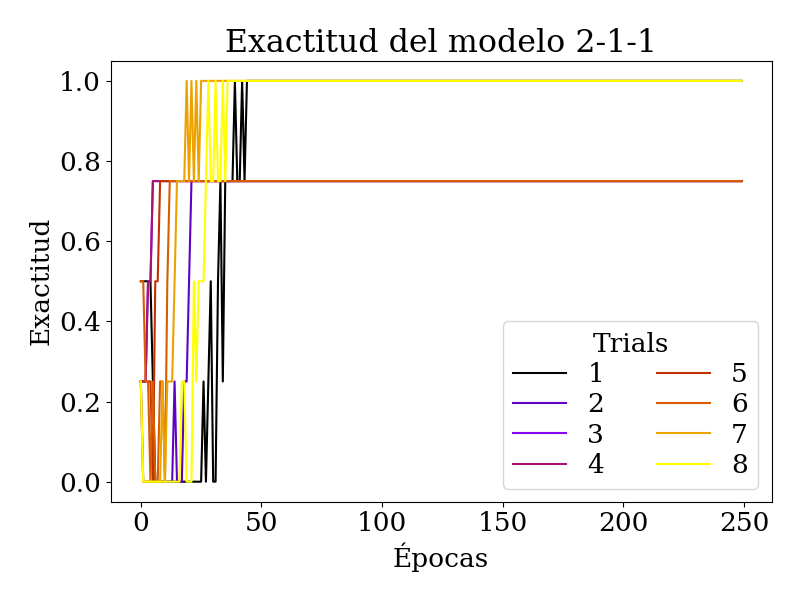
\includegraphics[width=0.44\textwidth]{../Graficos/ejer_1_2-1-1_acc.png}
	\caption{Exactitud en función de las épocas para la arquitectura 2-1-1.}
	\label{fig:XOR_acc_211}
\end{figure}


\section*{Ejercicio 2: XOR generalizado}

A diferencia del ejercicio anterior del XOR, ahora la función tiene N entradas, N$'$ neuronas en la capa oculta conectadas a las entradas, y una salida conectadas a todas las neuronas de la capa oculta, además de entradas adicionales para simular los umbrales . Esta arquitectura se muestra en la Fig.\,\ref{fig:arq-NN1}. La salida es $+1$ si el producto de las N entradas es $+1$ y $-1$ si el producto de las entradas es $-1$. Al igual que el ejercicio anterior, se utilizó la función $tanh(x)$ como función de activación.

\begin{figure}[H]
	\centering
	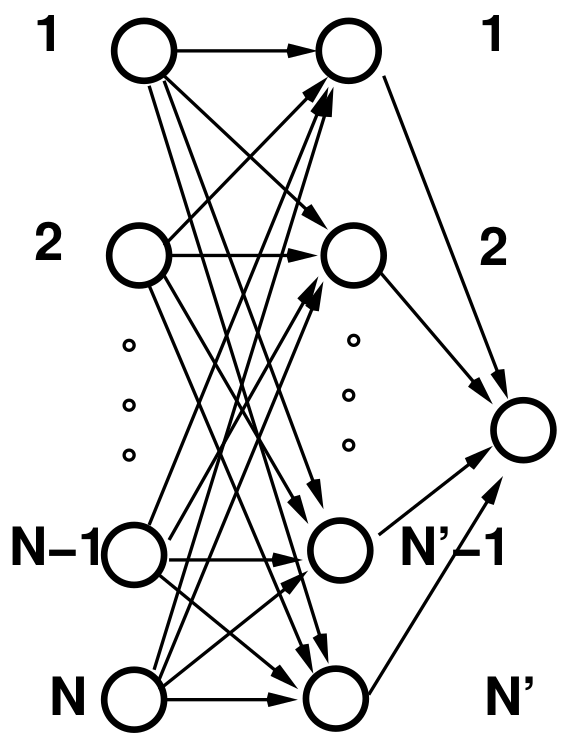
\includegraphics[width=0.15\textwidth]{ejer_2_NN1.png}
	\caption{Arquitectura N- N$'$ -1}
	\label{fig:arq-NN1}
\end{figure}

\subsection*{Pérdida y exactitud en función de la época}

Para esta sección utilizaremos la nomenclatura $(N, N', N_{train})$ para referirnos a la cantidad de entradas N, de neuronas en la capa oculta $N'$ y la cantidad de ejemplos para el entrenamiento $N_{train}$. Una vez definido estos parámetros, se ejecuta el programa con valores iniciales aleatorios para los pesos y los umbrales. En la Fig.\ref{fig:XOR_N_los} se muestra la pérdida en función de las épocas para distintas ejecuciones del programa con distintos valores para $N$, $N'$ y $N_{train}$. Se observa que para la pérdida tiene a ser nula para la mayoría de los casos en las primeras $250$ épocas, excepto para $(4,1,16)$, $(4,3,16)$ y $(7,4,100)$.

\begin{figure}[H]
	\centering
	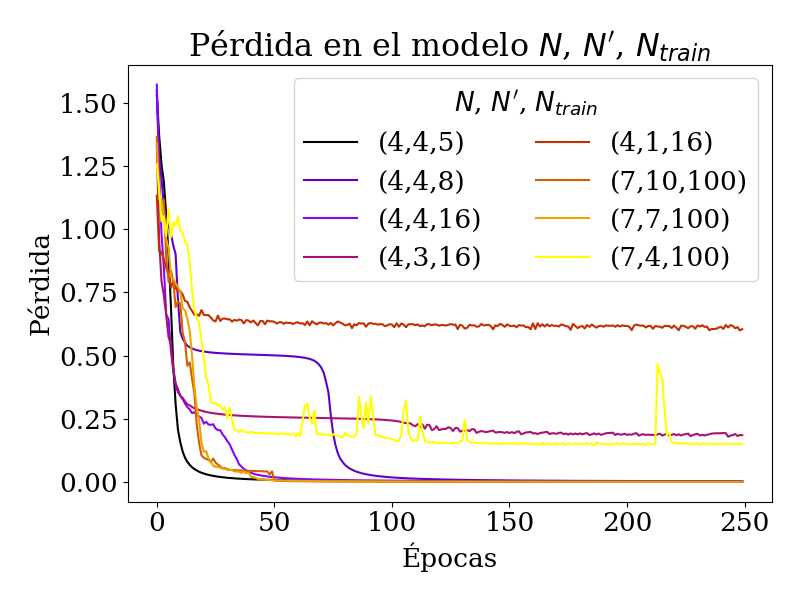
\includegraphics[width=0.45\textwidth]{../Graficos/ejer_2_los.png}
	\caption{Pérdida en función de la época para distintas arquitecturas}
	\label{fig:XOR_N_los}
\end{figure}

En los casos donde la pérdida no tiene a $0$, si consideramos la exactitud de los mismos tal como se muestra en la Fig.\,\ref{fig:XOR_N_acc}, la misma no tiende a ser $1$. Esto se debe a la presencia de mínimo locales en la convergencia.
\begin{figure}[H]
	\centering
	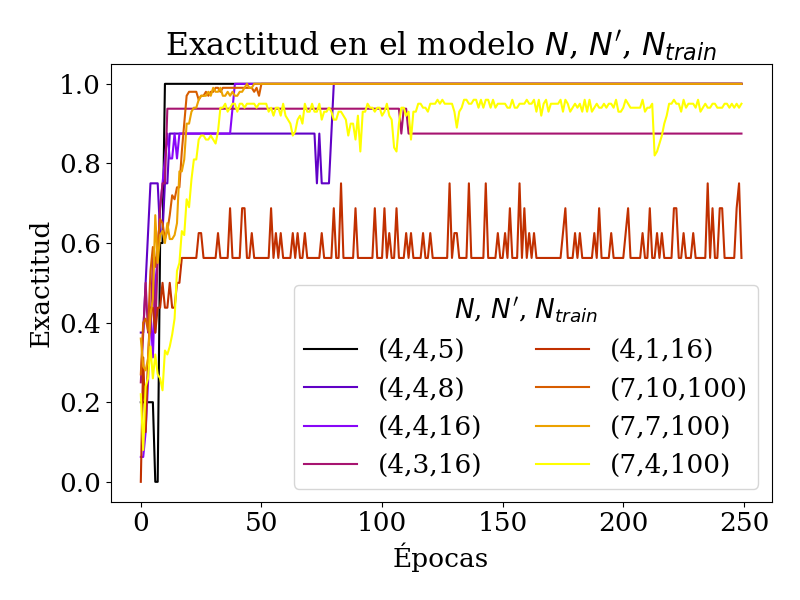
\includegraphics[width=0.45\textwidth]{../Graficos/ejer_2_acc.png}
	\caption{Exactitud en función de la época para distintas arquitecturas}
	\label{fig:XOR_N_acc}
\end{figure}
 Para los casos   $(4,4,16)$, $(4,3,16)$ y $(4,1,16)$, se entrena la red con todas las combinaciones posibles del XOR generalizado para 4 entradas. La diferencia entre las mismas es la cantidad de neuronas en la oculta. Se observa que cuando $N>N'$ la red tarda más en converger que cuando $N<=N'$, por ejemplo $(7,4,100)$. Esto se debe a la dimensión del problema no es suficiente para separar a los puntos de entrenamiento, como se espera con un perceptron.

\section*{Ejercicio 3: Mapeo Logístico }

La función que la red neuronal busca solución es conocida, que la función logística, dada por la Ec.\,\ref{eq:logistica} del tipo 
\begin{equation}
	x(t+1) = 4x(t)(1-x(t)).
	\label{eq:logistica}
\end{equation}
Para generar los valores de entrenamiento, se define la cantidad de épocas $T$ en las que los pesos van a actualizar. Con este valor, se calcula $x(T)$ usando como valor inicial $x[T-1]$ un valor aleatorio en el intervalo $(0,1)$.

La arquitectura utilizada se muestra en la Fig.\,\ref{fig:arq-mapeo}. En la ejecución del programa se agregaron neuronas adicionales para simular los umbrales y es utilizó un valor de $\eta=0.05$. 
\begin{figure}[H]
	\centering
	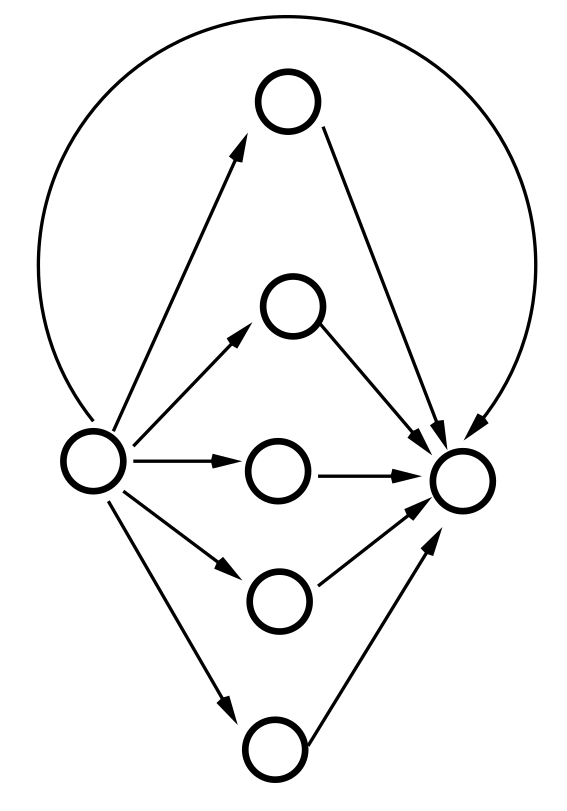
\includegraphics[width=0.15\textwidth]{ejer_3.png}
	\caption{Arquitectura para regresionar la función de mapeo logístico.}
	\label{fig:arq-mapeo}
\end{figure}

\subsection*{Error en función de la época}

Durante la evolución   de la red, se presentaron 15 ejemplo para verificar el error generalización en función de las épocas comparada con el error de entrenamiento, como se muestra en la Fig.\,\ref{fig:log_los_gen}. Se observa que para 5 ejemplos de entrenamiento, el error de entrenamiento, representada por una línea continua, converge a un valor no nulo en las primeras $250$ épocas, mientras que el error de generalización, mostrada como una línea punteada, tiende a seguir disminuyendo. En cambio para 10 ejemplos de entrenamiento, ambos error disminuyen y la diferencia entre ambos disminuye en función de las épocas. Ya para $100$ ejemplos, ambos errores convergen rápidamente a 0, esto se debe a la cantidad de ejemplos de entrenamiento que usa la red para actualizar sus pesos.


\begin{figure}[H]
	\centering
	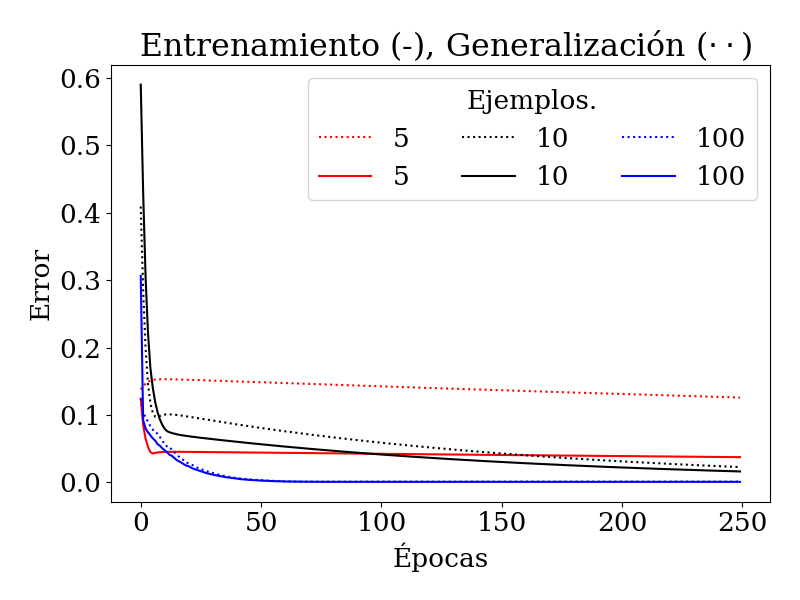
\includegraphics[width=0.5\textwidth]{../Graficos/ejer_3_los_gen.png}
	\caption{Error en función de la época para distintas cantidades de ejemplos de entrenamiento.}
	\label{fig:log_los_gen}
\end{figure}

\end{document}